%%%%%%%%%%%%%%%%%%%%%%%%%%%%%%%%%%%%%%%%%
% "ModernCV" CV and Cover Letter
% LaTeX Template
% Version 1.3 (29/10/16)
%
% This template has been downloaded from:
% http://www.LaTeXTemplates.com
%
% Original author:
% Xavier Danaux (xdanaux@gmail.com) with modifications by:
% Vel (vel@latextemplates.com)
%
% License:
% CC BY-NC-SA 3.0 (http://creativecommons.org/licenses/by-nc-sa/3.0/)
%
% Important note:
% This template requires the moderncv.cls and .sty files to be in the same 
% directory as this .tex file. These files provide the resume style and themes 
% used for structuring the document.
%
%%%%%%%%%%%%%%%%%%%%%%%%%%%%%%%%%%%%%%%%%
%---------------------------------------------------
%	PACKAGES AND OTHER DOCUMENT CONFIGURATIONS
%---------------------------------------------------

\documentclass[10pt,a4paper,sans]{moderncv} % Font sizes: 10, 11, or 12; paper sizes: a4paper, letterpaper, a5paper, legalpaper, executivepaper or landscape; font families: sans or roman

\moderncvstyle{casual} % CV theme - options include: 'casual' (default), 'classic', 'oldstyle' and 'banking'
\moderncvcolor{green} % CV color - options include: 'blue' (default), 'orange', 'green', 'red', 'purple', 'grey' and 'black'

\usepackage{lipsum} % Used for inserting dummy 'Lorem ipsum' text into the template
\usepackage{}
\usepackage{wrapfig}
\usepackage{multicol}
\usepackage[scale=0.85]{geometry} 
\usepackage{hyperref}
\hypersetup{
    colorlinks=true,
    linkcolor=blue,
    filecolor=magenta,      
    urlcolor=blue,
}
\urlstyle{same}
% Reduce document margins
%\setlength{\hintscolumnwidth}{3cm} % Uncomment to change the width of the dates column
%\setlength{\makecvtitlenamewidth}{10cm} % For the 'classic' style, uncomment to adjust the width of the space allocated to your name

%------------------------------------------------
%	NAME AND CONTACT INFORMATION SECTION
%------------------------------------------------

\firstname{Mohammad Reza} % Your first name
\familyname{Haghighat} % Your last name

%------------------------------------------------

\begin{document}
	%--------------------------------------------
	%	CURRICULUM VITAE
	%--------------------------------------------
	\makecvtitle % Print the CV title
	\vspace{-15mm}
    \begin{multicols}{2}
	    \section{Personal Information}
	        \cvitem{Full Name}{Mohammad Reza Haghighat}
	        \cvitem{Date of birth}{21.9.1985}
	        \cvitem{Nationality}{Iran}
	        \cvitem{Cellphone}{+98 912 542 64 41}    
	        \cvitem{Address}{Parvin Etesami ave. 21, Zanjan, Iran}
	        \cvitem{Email}
	        {
	            \href{mailto:haghighatmr@gmail.com}{haghighatmr@gmail.com}
	        }
            \hspace{6cm}
            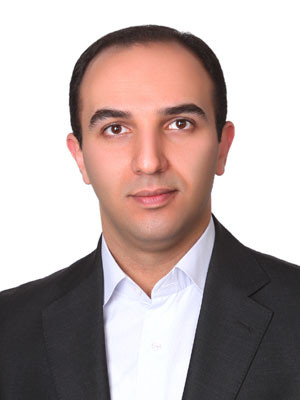
\includegraphics[width=.28\linewidth]{MRH}
    \end{multicols}
    %------------------------------------------
	%	Research Interest
	%------------------------------------------
    \section{Profile Summary}
	    \cvitem{}
	    {
	        Driven technical manager and senior software developer with 9+ years experience in software architecture, design, and development. Skilled at Data Discovery tools and Data mining, having delivered around 10 successful commercial projects in enterprise scale. After graduating in 2010 with a BSc degree in Computer Science \& Software Engineering, I started working at renowned software/IT companies in Iran while in parallel pursuing my own entrepreneurial enthusiasm. In December 2013 I founded my own software tech company, SimiaTec Co., for which I serve as the CEO at the moment. Currently a lecturer at the University of Applied Science \& Technology in Zanjan, Iran, I have additionally gained experience training over 60 personnel for my own company throughout the past 6 years. I learned to work in a team from day one and have experienced the entire spectrum of the team-working from a junior member to a group leader. I am now determined to undertake a PhD as an invaluable experience in independent research. 
	    }
	%--------------------------------------
	%	Research Interest
	%--------------------------------------
    \section{Research Interests}
	    \cvitem{}
	    {
	        Embedded Systems,
	        IoT,
	        Operating Systems,
	        Agile Methodologies,
	        Data Analysis
	       \iffalse{ \textbf{B}usiness \textbf{I}ntelligent}\fi
	    }
	%-------------------------------------
	%	EDUCATION SECTION
	%-------------------------------------
    \section{Education}
	    \cventry{2006--2010}
	        {BSc}
	        {\textbf{Computer Science-Software Engineering}}
	        {Azad University}{Zanjan, Iran}{}
	%--------------------------------------
	%	Employment
	%--------------------------------------
    \section{Employment}
	    \cventry{2018--Present}
	        {Founder \& CEO}
	        {\href{http://intl.irannsr.org/}{SimiaTec Co}}
	        {}{}{}	
	    \cventry{2017--Present}
	        {Senior Consultant}
	        {\href{http://intl.irannsr.org/}{Iranian ICT Guild Organization}}
	        {}{}{}	
	    \cventry{2016--Present}
	        {Board Member}
	        {\href{http://arian.co.ir/en-us/home-page}{Arian Novin Co}}
	        {}{}{}	
	    \cventry{2016--2018}
	        {Technical Manager}
	        {\href{http://arian.co.ir/en-us/home-page}{Arian Novin Co}}
	        {}{}{}	
	    \cventry{2015--2018}
	        {Senior Software Engineer \& DBA}
	        {\href{http://arian.co.ir/en-us/home-page}{Arian Novin Co}}
	        {}{}{}	
	    \cventry{2014--2015}
	        {Senior Software Engineer}
	        {\href{http://arian.co.ir/fa-ir/}{Zarrin Co}}
	        {}{}{}	
	    \cventry{2012--2014}
	        {Senior IT Advisor}
	        {\href{https://www.ghbi.ir/fa/}{Ghavamin Bank}}
	        {}{}{}	
	    \cventry{2010--2012}
	        {Software Engineer}
	        {\href{https://www.systemgroup.net/}{Hamkaran Co}}
	        {}{}{}	
	

	%----------------------------------------
	%	Teaching Experience
	%----------------------------------------
	\section{Teaching Experience}
	    \cvitem{}
	    {
	        \textbf{Lecturer} at the \href{https://www.uast.ac.ir/en}{University of Applied Science and Technology}, Zanjan, Iran, for the courses:
	    }
	    \begin{multicols}{2}
		        \cvitem{$\bullet$}
		        {
		            Software Engineering Concepts, Since 2015
		        }
		        \cvitem{$\bullet$}
		        {
		            Object Oriented principles, Since 2015
		        }
		        \cvitem{$\bullet$}
		        {
		            C/C++ basic \& advanced, Since 2014
		        }
		        \cvitem{$\bullet$}
		        {
		            C\#.net basic \& advanced, Since 2016
		        }
		        \cvitem{$\bullet$}
		        {
		            Database Design basic \& advanced, Since 2014
		        }
		        \cvitem{$\bullet$}
		        {
		            Data Science advanced, Since 2014
		        }
		        \cvitem{$\bullet$}
		        {
		            Full Stack MERN, Since 2018
		        }
	        \end{multicols}
	        \cvitem{}
	        {
	            \textbf{Speaker} for the workshops:
	        }
		        \cvitem{$\bullet$}
		        {
		            Organization Architecture, \href{http://agrizanjan.ir/mainenglishpage}{Agricultural Reform Organization}, Zanjan, Iran, 2016
		        }
		        \cvitem{$\bullet$}
		        {
		            Team Building \& Team Leading, \href{https://www.uast.ac.ir/en}{University of Applied Science and Technology}, Zanjan, Iran, 2018
		        }
		        \cvitem{$\bullet$}
		        {
		            Data Discovery, \href{http://zums.ac.ir/index.php?slc_lang=en&sid=1}{Zanjan University of Medical Sciences}, Zanjan, Iran, 2018
		        }
	%--------------------------------------
	%	Technical Skills
	%--------------------------------------
	\section{Technical Skills}

\begin{tabular}{}
    \cventry{Programming}
    {
        \begin{itemize}
            \item Experienced in VB.net - Since 2005
            \item Proficient in C/C\texttt{++} -\t Since 2007
            \item Experienced in Java - Since 2007
            \item Proficient in SQL - Since 2008
            \item Experienced in UML - Since 2009
            \item Proficient in C\#.net - Since 2010 
            \item Proficient in HTML - Since 2010
            \item Proficient in JavaScript - Since 2012
            \item Proficient in React.Js - Since 2014
            \item Experienced in BPMN2.0 - Since 2017
        \end{itemize}
    }{}{}{}{}
\multicolumn{2}{c}{} \\
%------------------------------------------------

\textsc{Technical Software \t} & \begin{itemize}
  \item Proficient in Visual Studio - Since 2003
  \item Proficient in MS SQL Server - Since 2007
  \item Proficient in Visio - Since 2009
  \item Proficient in Git - Since 2015
  \item Proficient in VSCode - Since 2018
  \item Proficient in Qlik view - Since 2018
  \item Proficient in Power BI - Since 2018
  \item Experienced in Microsoft Team Foundation - Since 2018
  \item Experienced in MonoDB - Since 2019
  \item Experienced in Cassandra - Since 2019
\end{itemize}\\
\multicolumn{2}{c}{} \\
%------------------------------------------------

\textsc{Technologies \t} & \begin{itemize}
  \item Proficient in SSIS (SQL Server Integration Services)  - Since 2017
  \item Proficient in SSAS (SQL Server Analysis Services)  - Since 2017
  \item Proficient in SSRS (SQL Server Reporting Services)  - Since 2017
  \item Proficient in OLAP - Since 2017
  \item Proficient in ETL - Since 2017
\end{itemize}\\
\multicolumn{2}{c}{} \\
\end{tabular}

	%------------------------------------
	%	Projects
	%------------------------------------
	\section{Projects}
        \cvitem{$\bullet$}
        {
            Design \& development of an \textbf{Offline Payment System} to manage the cost of using urban services, such as taxis, buses, playgrounds, recreational facilities, etc. Using RFID technology \& Myfare cards, \textcolor{red}{??I/we/me and my team of five??} implemented the project for the \href{https://www.zanjan.ir/}{Zanjan Municipality} which operated for over 5 years in 2 provinces of Iran \textcolor{red}{which tow??}. Developed by .Net technology (2010 to 2015)
        }
        \cvitem{$\bullet$}
        {
            Design \& development of an \textbf{Asset Tracking System}, as a government funded project for managing fixed assets and inventory controls in the IoT platforms using RFID tags. The framework includes a central database \text{(MS SQL Server)}, a desktop application \text{(.Net Windows Form App)} and a software for a hand-held device \text{(Windows CE based App)}. Operated in 2 government offices of Iran for over 3 years, \href{http://zanjan.isiri.gov.ir/Portal/Home/}{Institute of Standards and Industrial Research of Iran, Zanjan Branch} and \href{http://www.intamedia.ir/Pages/Action/Province/tax29}{head office of tax Affairs}. (2011 to 2014)
        }
        \cvitem{$\bullet$}
        {
            Implemented a \textbf{Statistical Data Collector \& Monitoring Dashboard} Development for \href{https://www.ghbi.ir/fa/}{Ghavamin  financial and credit institution} in private sector.A financial and credit institution that has many branches wants to collect and visualize their daily performance data on e-forms and management dashboard, this web-based system was developed on React.js platform and used for 4 years. (2011 to 2015)
        }
        \cvitem{$\bullet$}
        {
            Implemented a \textbf{Reliable Auto Backup system} Development for \href{https://www.ghbi.ir/fa/}{Ghavamin Bank} in semi private sector. The organization has several Fox-Pro Database servers in different Geo-locations. This system developed as a local service and a central server application. that responsible for taking a differential backup, merging them to the archive, and guaranteed that always the latest and valid backup for any database is available. (2012 till Now)
        }
        \cvitem{$\bullet$}
        {
            Implemented a \textbf{Dynamic e-form Generator} Development as a part of BPMS project. A government project for the \href{http://zn.mefa.ir/}{Main Office of the Economy of Zanjan Province}, to collect monthly statistical data from 25 other government agencies. For validation, Verification and centralized data storage. That data forms were dynamically designed and released to others on the Web. Later, this software was added to a BPM suite. (2016-2017)
        }
        \cvitem{$\bullet$}
        {
            Project management, to implement a \textbf{Chart library on .NET} as part of a government requirement for \href{http://zn.mefa.ir/}{Main Office of the Economy of Zanjan province}, BPM project. (2017)
        }
        \cvitem{$\bullet$}
        {
            Managing \& planning a \textbf{Dynamic Dashboard Generator} application as analyzer \& project manager for operation in a zinc ingot factory to manage data exchange between different manufacturing units. To validate data in different origins and better management of production and supply. Data from different databases was collected and displayed on a dashboard after entering to a data warehouse. For non-electronic inputs, dynamic forms were created with the molding tool. (2017-2018)
        }
        \cvitem{$\bullet$}
        {
            Managing \& planning a \textbf{Business Process Management System} as Database designer\& system architecture \& project manager for  \href{http://sama.mefa.ir/Portal/Home/default.aspx}{Iran Ministry of Economic Affairs and Finance}, to managing inter-agency interactions and issuing electronic licenses. (2017-2018)
        }
    	\cvitem{$\bullet$}
    	{
    	    Design \& Developed a \textbf{Statistical Analyzer \& Competitive Smart System} for strategic KPI tracking. for , \href{http://qo.mefa.ir/}{Main Office of the Economy of Qom} and \href{http://mk.mefa.ir/}{Markazi} Provinces, \href{https://cfu.ac.ir/}{Main Office of Farhangian University} in Tehran and \href{http://zzkico.ir/en-us/Home/groups/15}{Zanjan Zinc Khales Sazan} in private sector, for strategic business monitoring and management dashboards, based on predefined plans and strategies. Will be able to receive key indicators of each strategy, then adapt it to an operational plan and report the diversion rate. The most important key feature is tracking the parameters involved in the deviations. This system contributes to the major decisions of an organization. (2018)
    	}
	
	%---------------------------------------------
	%	LANGUAGES SECTION
	%---------------------------------------------
	\section{Languages}
        \begin{multicols}{2}
		    \cvitem {Persian:}{Native}
		    \cvitem {English:}{Proficient, C1}
        \end{multicols}
        
	%---------------------------------------------
	%	References
	%---------------------------------------------
	\section{References}
        \begin{multicols}{2}
		    \cvitem {Ref1}{name and contact}
		    \cvitem {Ref2}{name and contact}
        \end{multicols}
\end{document}
